\documentclass{IEEEtran}
\usepackage{graphicx}
\usepackage{listings}
\usepackage{amsmath}
\usepackage{cite}
\usepackage{booktabs}
\usepackage{xcolor}
\markboth{Sentiment Analysis of News Entities in Armenia}{Movsisyan: Title}
\definecolor{codegreen}{rgb}{0,0.6,0}
\definecolor{codegray}{rgb}{0.5,0.5,0.5}
\definecolor{codepurple}{rgb}{0.58,0,0.82}
\definecolor{backcolour}{rgb}{0.95,0.95,0.92}

\lstdefinestyle{mystyle}{
    backgroundcolor=\color{backcolour},   
    commentstyle=\color{codegreen},
    keywordstyle=\color{magenta},
    numberstyle=\tiny\color{codegray},
    stringstyle=\color{codepurple},
    basicstyle=\ttfamily\footnotesize,
    breakatwhitespace=false,         
    breaklines=true,                 
    captionpos=b,                    
    keepspaces=true,                 
    numbers=left,                    
    numbersep=5pt,                  
    showspaces=false,                
    showstringspaces=false,
    showtabs=false,                  
    tabsize=2
}

\lstset{style=mystyle}

\usepackage[T1]{fontenc}
\usepackage[utf8]{inputenc}
\author{Mher Movsisyan \\ BS in Data Science American University of Armenia Yerevan, Armenia\\ mher\_movsisyan.\@edu.aua.am\\[1cm]{\small Advisor: Rafael Shirakyan\\ rshirakyan\@gmail.com}}
\title{Sentiment Analysis of News Entities in Armenia}

\begin{document}
\maketitle

\begin{abstract}
The rapid proliferation of online news sources has led to a wealth of information that can be analyzed to gain insights into public sentiment and opinions about various entities and topics. \\
This paper aims to explore and harness the capabilities of OpenAI’s GPT-3.5, a large language model (LLM), as an easily accessible text processing component, specifically for sentiment analysis. We show the advantages and disadvantages of integrating an LLM as a component, we look for relationships among entities and build a methodologically simple sentiment estimator to infer the sentiment of all the entities within the scraped dataset.
\end{abstract}
{Key Words:}
News.am, Tert.am, Armenpress, news, sentiment analysis, LLM

\section{Introduction}

Sentiment analysis, also known as opinion mining, is a natural language processing (NLP) technique that involves determining the sentiment expressed in a piece of text, such as positive, negative, or neutral. It uses machine learning models to analyze and understand subjective information conveyed in written or spoken language (unstructured data), helping to gauge the sentiment or emotional tone of the text. This analysis is valuable in various applications, including social media monitoring, customer feedback analysis, and market research. There are various ways to perform sentiment analysis; In our case, we have articles in which more than one entity can be discussed, and each of those entities can have different sentiment. Inferring separate sentiments for each entity is a complex task that involves an ML system with components of tokenization, named entity recognition, context-aware attribute linking and sentiment analysis just to name a few. Commercially available LLMs provide an easy workaround to this methodological complexity, and will allow one-person teams of researchers to explore what would otherwise take several months for entire departments.
\newline
\newline
The primary objectives of this research are to:
\begin{itemize}
    \item collect news articles from Armenian media sources,
    \item utilize GPT3.5 (gpt-3.5-turbo-1106) to extract entities mentioned in the news articles,
    \item conduct sentiment analysis on the extracted entities,
    \item aggregate sentiment data over time to create a time-series dataset,
    \item analyze the data to determine if there are significant differences in the sentiments expressed toward the same entities between and across news sites,
    \item discuss the possible drawbacks and future research vectors of using LLMs as a means of natural language processing.
\end{itemize}



\section{Materials}
\textbf{The choice of what particular LLM to use} was based on the compatibility of the model with a component-like use case. OpenAI’s “gpt-3.5-turbo-1106” stood out among the alternatives by having a built-in feature of returning a JSON string as a response to a prompt, thus requiring less prompt engineering and providing more reliability in the structure of the response. The structure of the response is crucial, since the end-user is another component within a pipeline.



\section{Data Collection}

\textbf{Choosing which articles to collect} was a choice based purely on a cost-to-outcome basis. Only the articles written in English were chosen to be collected, which was done to mitigate costs, as Armenian texts are expensive to respond to (we will discuss why in the Discussion section).

\textbf{Choosing which news sites to conduct this study on} was based on the choice of which articles were to be collected. Only the news sites that produce articles in written English were chosen, more specifically: Tert.am, News.am, and Armenpress.

\textbf{The data collection process} was done by web scraping all the articles written in english from the three chosen news providers. This process consisted of two stages; First, the list of articles to-be-scraped and their corresponding uniform resource locators (URLs) were scraped totaling 14,253 pages, which took less than 3 hours of computation on a commercially available laptop (specifications provided in the appendix), most of which was network activity which again highlights the availability of the entire research process. Secondly, the date of publishing and content of 432,944 articles were scraped along with the “theme” that the article was classified as by the publisher, if it was provided. This process took less than 17 hours.


\begin{figure}
    \centering
    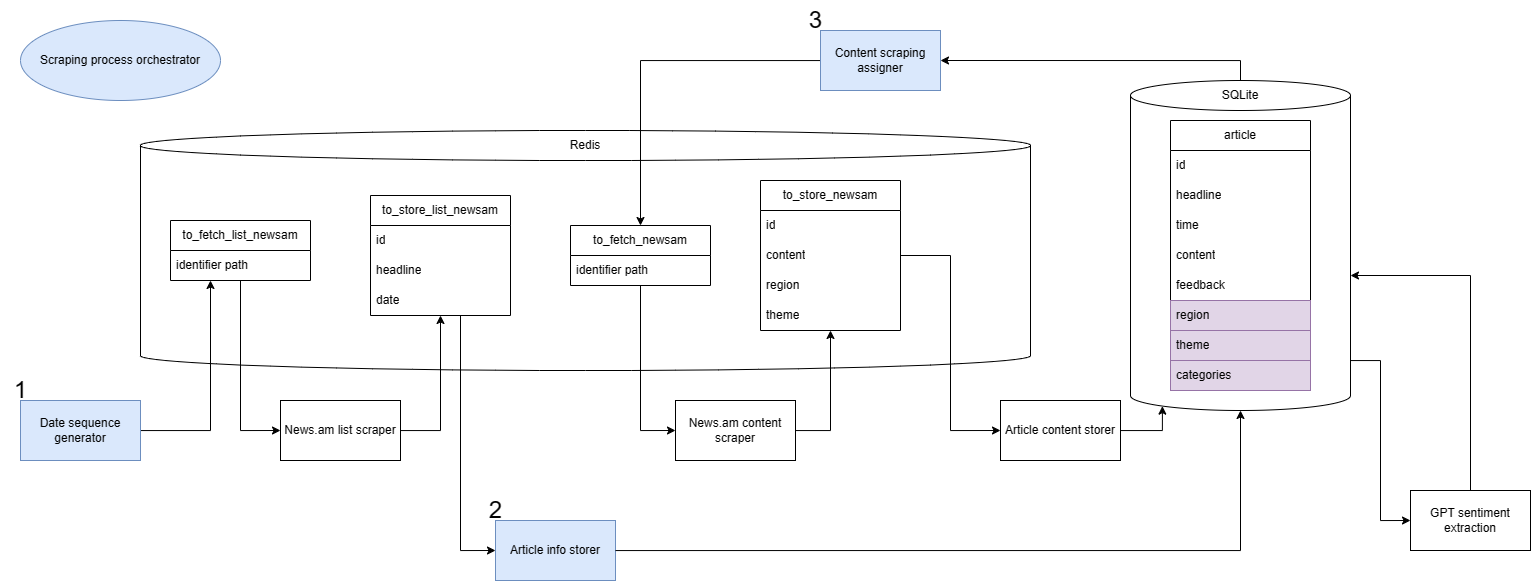
\includegraphics[width=1\linewidth]{flow.drawio.png}
    \caption{The process of data scraping}
    \label{fig:flow}
\end{figure}

\hspace

\section{Methodology}
\textbf{The choice of which entities to analyze the sentiment of across time} was based on arguably the two most prominent geopolitical forces within the region, Russia and the United States of America.

\textbf{Choosing which articles to extract sentiment from} was done by firstly limiting the number of articles from each news site to 16,000, then randomly sampling without replacement the articles that either contain “Russia” in their headline or “United States” in their content.

\textbf{The sentiment extraction process} was done by providing each article with the prompt

\lstinputlisting{prompt_sys.json}
\lstinputlisting{prompt_user.json}
One, but not the only reason why there is an additional “explanation” field, is that LLMs tend to perform better when they are asked to explain their answer (Kojima et al. 1).\newline

\textbf{A sentiment aggregation process} was put in place to attribute the entirety of the sentiment of each article to a single entity (either Russia or USA). This is done by first counting the number of times any entity is given a sentiment of “positive”, “negative” or “neutral” for each article, then dividing that by the total number of entities within the article. The sentiment with the highest ratio will be assigned to the article, and if, for example, an article regarding Russia is assigned a neutral sentiment, this sentiment will be considered to be representative of the sentiment of Russia within the article. This is done to account for both Russia and the US being a multi-faceted entity represented by and closely associated with several physical entities such as presidents, diplomats, and other entities.

\textbf{For analysis}, we chose the Wilcoxon signed-rank test when checking for significant differences between entity sentiment in one news site. We chose the Friedman chi squared test for checking if sentiment is similarly distributed between the years for one entity in one news site.

After the initial analysis, we \textbf{checked for the consistency of the responses} to our prompts, where some imperfections were found. For the details of the findings refer to the results section.

Then \textbf{the entities were parsed} into python dictionaries where the entity name was the key and the value was again a dictionary containing:
\begin{itemize}
    \item positive: number of times the entity was mentioned in positive sentiment,
    \item negative: number of times the entity was mentioned in negative sentiment,
    \item neutral: number of times the entity was mentioned in neutral sentiment,
    \item connections: a python list of three dictionaries which hold the number of positive, negative and neutral mentions within the same article. They are represented as yet another dictionary where the key is the second entities name and the value is the number of articles in which they co-occured.
\end{itemize}

A short example:
\lstinputlisting{example_entity.txt}

The parsed data was then used to check \textbf{whether or not it contains enough useful information for a commercial use-case}. Looking at the number of positive, negative, and neutral sentiment of each entity, one could get a general estimate of how a brand name is represented in the news media.

To parse the news landscape visually, a graph was constructed where each node is an entity, and the size is a function of the number of articles the entity was mentioned in (see figure 2).

\begin{figure}
    \centering
    \includegraphics[width=1\linewidth]{output.png}
    \caption{Entities as nodes, size as a function of occurrences}
    \label{fig:graph}
\end{figure}


To \textbf{infer the sentiment for the rest of the articles} without it costing us more financial resources, we opted for building a small and fast model. 

Firstly, in the part of the dataset which had feedback from the LLM, we checked for each entity name in the article. When the entity name was found, the sentences in which the entity was mentioned were selected, along with the explanation of the LLM regarding the sentiment. The words in those sentences and the explanation were then counted for each sentiment the entity was assigned. In the end, each word had three numbers associated with it: positive, negative and neutral occurrences. 
Then, when inferring the sentiment of an entity, we sum up those three numbers for all the words in the same sentence as the entity instance to get three numbers corresponding to each sentiment.
Beyond this point the method of inference splits into two ways:
\begin{enumerate}
    \item \textbf{The naive method}: We simply take the sentiment with the highest corresponding number as the inferred sentiment.
    \item \textbf{The weighted method}: We sum up the three numbers of all known words even if the word is not found in the sentence and use that sum as a divisor to the sentence sentiment sum, thus over-represented sentiments are are weighted down. Beyond this, we also multiply each sentence sentiment sum with a hyperparameter and tune it for accuracy.   
\end{enumerate}

We also ponder around the saying "Show me who your friends are, I'll tell you who you are" and the verse 1 Corinthians 15:33 "bad company corrupts good character" by \textbf{analysing second-degree and third-degree sentiments}.

First-degree sentiment of an entity is the sentiment assigned by the LLM. Second-degree sentiment of an entity is the mode sentiment among top 10 connections of the entity. Third-degree sentiment is the mode second-degree sentiment of the top 10 connections. Top 10 connections are the 10 entities which co-occur with the entity the most regardless of sentiment.


\section{Results}

The initial analysis questions yielded positive results for most of the tests that were conducted. 
\newline

\textbf{Question}: Do entities have different sentiments between each other within a news site? (see Table 1) 

Null Hypothesis $H_0$: There is no significant difference in sentiment between entities within a news site.  

Alternative Hypothesis $H_1$: There is a significant difference in sentiment between entities within a news site.

$\alpha = 0.01$

\begin{table}
    \centering
    \begin{tabular}{ccccc}
        Significance & p-value & statistic & sentiment & News site \\
        True & 2.205 * $10^{-20}$ & 34347 & positive & Armenpress \\
        True & 1.052 * $10^{-20}$ & 64104.5 & neutral & Armenpress \\
        True & 7.303 * $10^{-20}$ & 16251.5 & negative & Armenpress \\
        True & 3.621 * $10^{-20}$ & 33115.5 & positive & News.am \\
        True & 2.666 * $10^{-20}$ & 64133 & neutral & News.am \\
        True & 9.004 * $10^{-20}$ & 35911 & negative & News.am \\
        True & 5.263 * $10^{-20}$ & 30399.5 & positive & Tert.am \\
        True & 4.638 * $10^{-20}$ & 46969 & neutral & Tert.am \\
        False & 0.23 & 53159 & negative & Tert.am \\
        True & 2.781 * $10^{-20}$ & 198599.5 & positive & All together \\
        True & 5.366 * $10^{-20}$ & 426997 & neutral & All together \\
        True & 3.199 * $10^{-20}$ & 216308.5 & negative & All together \\
    \end{tabular}
    \caption{Wilcoxon test results}
    \label{tab:wilcoxon}
\end{table}

\begin{figure}
    \centering
    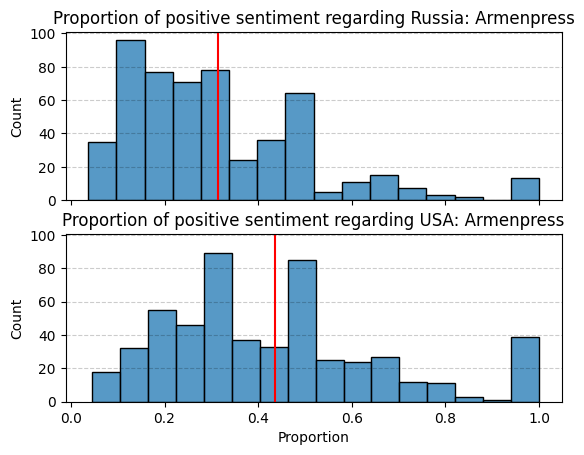
\includegraphics[width=1\linewidth]{figures/sig1.png}
    \caption{Histogram with red line indicating mean}
    \label{fig:positive_russia_armenpress}
\end{figure}

\begin{figure}
    \centering
    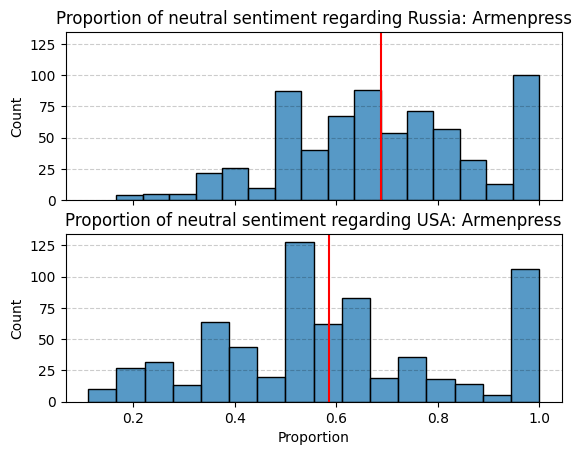
\includegraphics[width=1\linewidth]{figures/sig2.png}
    \caption{Histogram with red line indicating mean}
    \label{fig:neutral_russia_armenpress}
\end{figure}


\begin{figure}
    \centering
    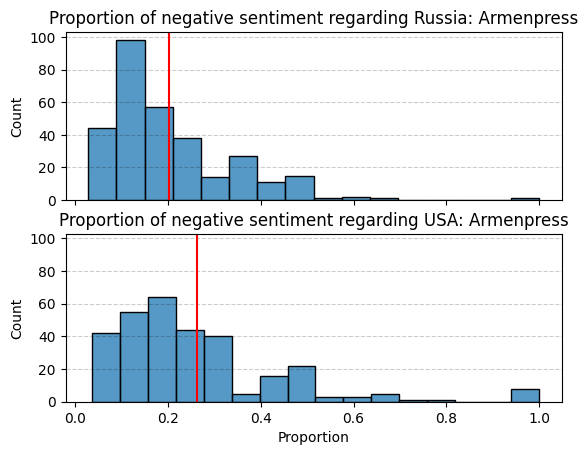
\includegraphics[width=1\linewidth]{figures/sig3.png}
    \caption{Histogram with red line indicating mean}
    \label{fig:negative_russia_armenpress}
\end{figure}


\begin{figure}
    \centering
    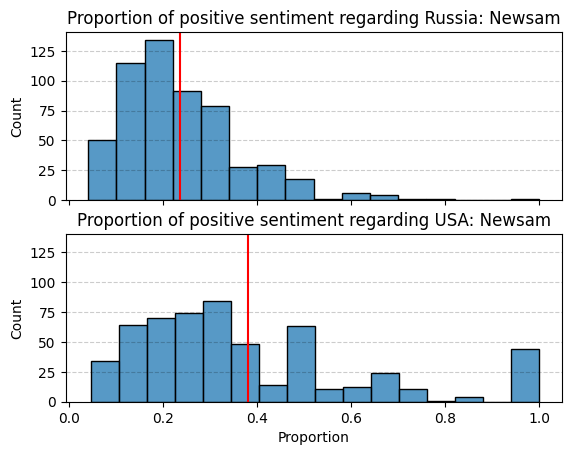
\includegraphics[width=1\linewidth]{figures/sig4.png}
    \caption{Histogram with red line indicating mean}
    \label{fig:positive_russia_newsam}
\end{figure}


\begin{figure}
    \centering
    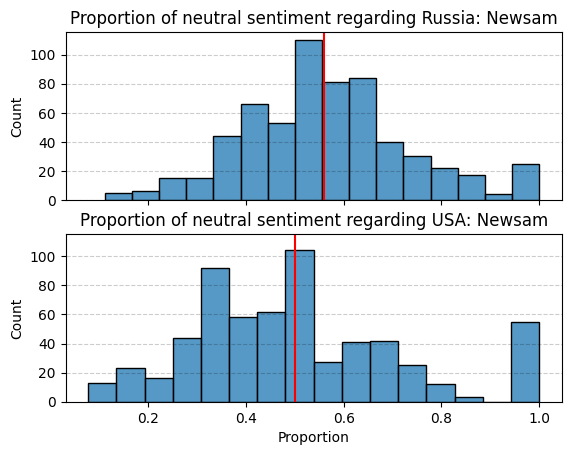
\includegraphics[width=1\linewidth]{figures/sig5.png}
    \caption{Histogram with red line indicating mean}
    \label{fig:neutral_russia_newsam}
\end{figure}


\begin{figure}
    \centering
    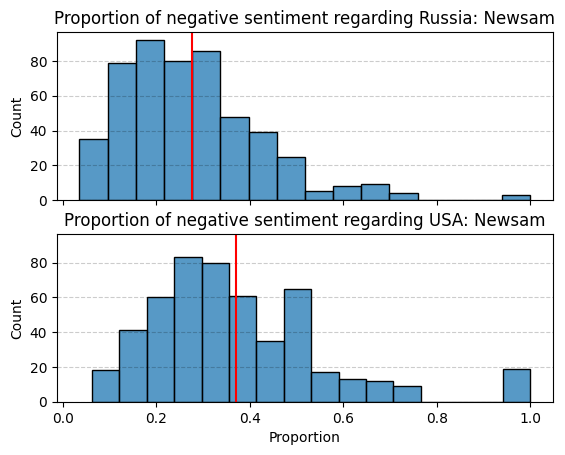
\includegraphics[width=1\linewidth]{figures/sig6.png}
    \caption{Histogram with red line indicating mean}
    \label{fig:negative_russia_newsam}
\end{figure}


\begin{figure}
    \centering
    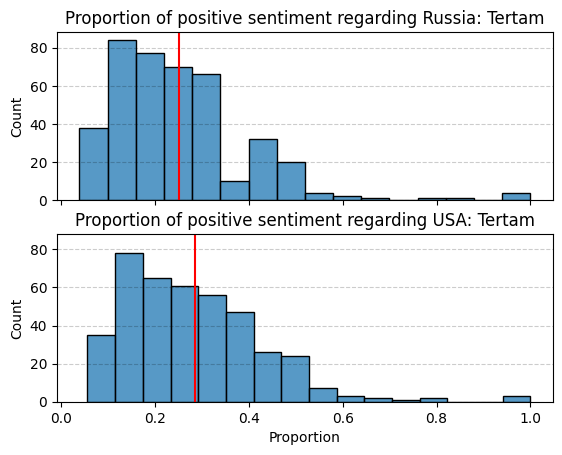
\includegraphics[width=1\linewidth]{figures/sig7.png}
    \caption{Histogram with red line indicating mean}
    \label{fig:positive_russia_tertam}
\end{figure}


\begin{figure}
    \centering
    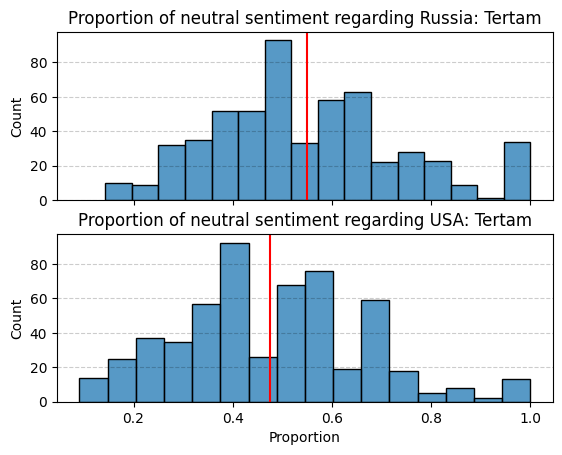
\includegraphics[width=1\linewidth]{figures/sig8.png}
    \caption{Histogram with red line indicating mean}
    \label{fig:neutral_russia_tertam}
\end{figure}


\begin{figure}
    \centering
    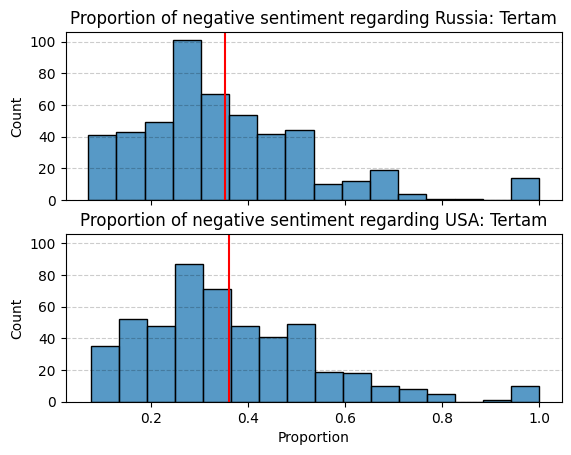
\includegraphics[width=1\linewidth]{figures/sig9.png}
    \caption{Histogram with red line indicating mean}
    \label{fig:negative_russia_tertam}
\end{figure}


\begin{figure}
    \centering
    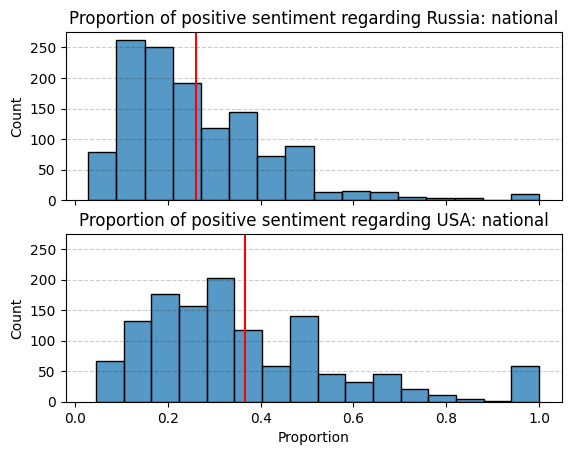
\includegraphics[width=1\linewidth]{figures/sig10.png}
    \caption{Histogram with red line indicating mean}
    \label{fig:positive_russia_national}
\end{figure}


\begin{figure}
    \centering
    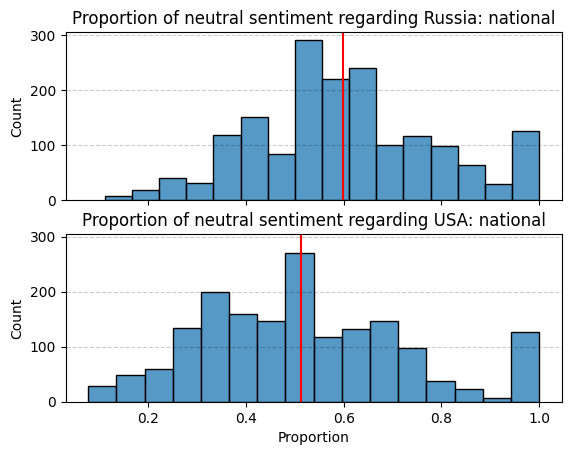
\includegraphics[width=1\linewidth]{figures/sig11.png}
    \caption{Histogram with red line indicating mean}
    \label{fig:neutral_russia_national}
\end{figure}

\begin{figure}
    \centering
    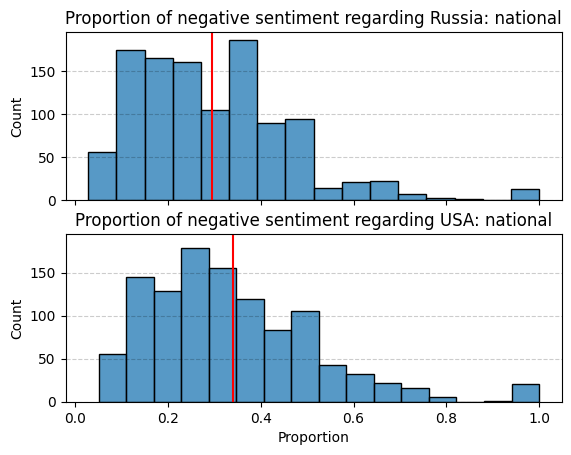
\includegraphics[width=1\linewidth]{figures/sig12.png}
    \caption{Histogram with red line indicating mean}
    \label{fig:negative_russia_national}
\end{figure}

\vspace{0.5cm}

\textbf{Question}: Entities have different sentiment throughout time within a news site. (see Table 2 and 3)

Null Hypothesis ($H_0$): There is no significant difference in sentiment for entities over time within a news site.  

Alternative Hypothesis ($H_1$): There is a significant difference in sentiment for entities over time within a news site  

Friedman chi square test with $\alpha = 0.01$


\begin{table}
    \centering
    \begin{tabular}{ccc}
        Source & statistic & p-value \\
        Armenpress & 151.20 & 1.179 * $10^{-25}$ \\
        News.am & 132.54 & 6.523 * $10^{-22}$ \\
        Tert.am & 351.27 & 4.203 $10^{-67}$ \\
    \end{tabular}
    \caption{Friedman chi-square test: Russia}
    \label{tab:friedman_russia}
\end{table}

\begin{table}
    \centering
    \begin{tabular}{ccc}
        Source & statistic & p-value \\
        Armenpress & 127.26 & 7.336 * $10^{-21}$ \\
        News.am & 104.25 & 2.480 * $10^{-16}$ \\
        Tert.am & 251.35 & 3.363 * $10^{-46}$ \\
    \end{tabular}
    \caption{Friedman chi-square test: USA}
    \label{tab:friedman_usa}
\end{table}

The figures 3 to 14 are aggregated for the unit of count to be one week, thus the proportion indicates the proportion of articles of the given category in one week.

\vspace{1.4cm}
\textbf{Consistency and ease of integration into larger systems of LLMs}
The component-like use case of \verb|gpt-3.5-turbo-1106| proved to contain imperfections. Out of the generated 36,827 article feedbacks that were to be in JSON format, 9 were not able to be parsed by \verb|ast.literal_eval|. In 8 of those cases the generated output failed to close the object/array with the respective syntactical symbol \verb|`| or \verb|]|.
\vspace{0.4cm}
\lstinputlisting{consistency.txt}

\textbf{Relationship mining}
The number of entities whose number occurrences are exceeding or equal to 10 are 1777. The number of total entities are 56945.

\textbf{Commercial usability}
The numbers show lack of useful information for most companies in Armenia, as the quantity of sentiments are not sufficient. For example American University of Armenia only has 4 positive and 2 neutral occurrences, and there are less than 10 OJSC (open joint-stock companies) entities, all of which lack sufficient number of sentiments for any practical analysis. 

\textbf{Inference results}
The number of articles inferenced are: 
\begin{verbatim}
'neutral': 3537606,
'positive': 545721,
'negative': 115134
\end{verbatim}
The naive estimator yielded an accuracy of 50.93\%, while the weighted estimator yielded an accuracy of 53.09\%

\textbf{Multi-degree sentiment analysis}
The second-degree sentiment coincided with the first-degree sentiment more than the estimators predictions, yielding a coincidence rate of 62.19\%, while the third-degree sentiment coincided with the first one 46.42\% of the time. The second-degree sentiment coincided with the third-degree sentiment 70.29\% of the time.



\section{Discussion}
The reason why LLMs are expensive for Armenian texts lies in the way that the models are trained. LLMs require text to be converted to tensors of numbers or tokens. But if we encode each letter as a separate token, the number of permutations for possible words increases exponentially and models have a hard time learning and storing representations. To fix this issue, a very effective way of tokenization is to group commonly occurring letters together. For example the word “token” can be tokenized into “to” and “ken”, where “to” is a commonly appearing group of letters. Entire words such as “day” or “tree” can be encoded as one token and thus save a lot of computational power. This is very handy if we are dealing with only one or few languages at a time. But when the training data includes a couple hundred languages, some are bound to be under/overrepresented due to the hasty data gathering and feeding techniques employed. Underrepresented languages will not be tokenized well, and in the case of Armenian, for the GPT-3.5 each letter is almost always the entire token. This greatly increases the cost to perform an inference request as the cost is a function of the number of tokens generated and the number of tokens in the prompt.

\section{Conclusion}
While the simple inference methods were a first-go-to methodologically simple ways of inferring sentiment, multi-degree sentiment analysis proved to be more reliable for this dataset. The LLM in use had good consistency in terms of the output structure, although additional checks and filters were needed to sift out non-compliant outputs. The commercial usability of the dataset is questionable at best. Additional data and sources are needed for a practical use case. The sentiment showed clear variation through time and across sources.

\bibliographystyle{IEEEtran}
\bibliography{references}
    [1] Kojima, Takeshi, et al. “Large Language Models are Zero-Shot Reasoners.” Computation and Language, vol. 0, no. 0, 2023, p. 0, https://arxiv.org/abs/2205.11916.



\end{document}